\documentclass{paper}
\usepackage{times}
\usepackage{geometry}
\geometry{letterpaper, portrait, margin=1in}
\usepackage{setspace} \doublespacing
\usepackage[utf8]{inputenc}
\usepackage{enumitem,amssymb}
\usepackage{ragged2e}
\usepackage{physics}
\usepackage{siunitx}
\sisetup{separate-uncertainty=true}
\usepackage{float}

\usepackage{caption}
\usepackage[hidelinks]{hyperref}
\usepackage{url}

\usepackage{graphicx}
\usepackage{epstopdf}
\usepackage{tikz}
\graphicspath{{data/concepts}}

\usepackage{aas_macros}
\usepackage[style=authoryear]{biblatex}
\bibliography{refs} %refs.bib
\nocite{*}

\immediate\write18{texcount \jobname.tex -out=\jobname.sum}

% set frameboxes to be borderless
\setlength{\fboxsep}{0pt}
\setlength{\fboxrule}{0pt}

\begin{document} 

\title{The constituents of the universe and the growth of structure}
\author{ariahayd}
\date{April 24, 2022}
\maketitle

% Overview. [8]
% Give an overview of the current standard model for the context of the essay. 
% Include one figure for this section. 
\section{Overview}
  The universe is shaped by its constituent energies, and its constituents are
  shaped by the size of space and the structures within it. The evolution of 
  the universe is understood through the Standard Model of Cosmology, 
  developed mainly over the last century of observations of matter and energy 
  on large scales, of galaxies and throughout \(Gpc^3\) volumes space, and on 
  the very small scales where the quantum mechanical properties of energy 
  fields emerge. 

  Today's most successful model is called \(\Lambda CDM\), the concordance
  model, with dynamics dominated by what can be explained through General 
  Relativity, Quantum Field Theory, and with contributions from Dark Energy 
  (\(\Lambda\)) and Cold Dark Matter (\(CDM\)). These last two components are 
  observationally confirmed but not entirely explained by theory. 

  The densities of energy in the fields within the universe determine the 
  geometry of space. \(\Lambda CDM\) requires a universal geometry curved by 
  the energy densities of these constituent fields. Observations indicate that 
  the curvature of the metric of spacetime over large distances is nearly 
  flat and has been throughout most of the history of the universe.
  
  In this model, the metric of the 
  universe is flat \(k=0\), and the equation of state parameter \(w\), that 
  energy to is 
  constant in time.

  The extent of space determines how structures evolve through through 
  different epochs of the Universe. 

  \begin{figure}[!htb]
    \begin{centering}
    \includegraphics[scale=1.0]{Intro-big_bang.pdf}
    \caption{A timeline of the hot big bang with times for each epoch,
      along with the average temperature, and average energy per particle.
    Credit: OpenStax, CC}
    \label{fig:Intro-big_bang}
    \end{centering}
  \end{figure}

  \(\Lambda CDM\) is based on a hot big bang origin of high energy density 
  that has since evolved to the today's universe of much lower density. The 
  standard model incorporates observations of evidence of important events 
  along the evoluationary history of the universe, evidence of phase changes 
  and 

  Among theories of the origin of the universe, the hot big bang is evidenced
  by the seemingly far distance to primordial quasar radio signals, and the
  lack of any nearby (\cite{Condon_1998}). 

  The big bang can be derived from an analysis of the metric of spacetime 
  applied to the universe in general. %include how einstein added lambda term


% 2. Dark Matter. [20]
% Describe two lines of evidence for dark matter. These should be distinct and 
% complementary. A line of evidence can consist of more than one observational 
% phenomenon that together provide the evidence. Include two figures for this 
% section.
\section{Dark Matter}
  Large, gravitationally bound systems such as galaxies and galaxy clusters 
  appear to be embedded in gravitational potentials deeper than expected given 
  the observable masses interacting within the system. The depth of these 
  potentials is inferred to be due to unobserved, \textit{dark} matter.

  % line of evidence one
  Early evidence for Dark Matter in the halo of a galaxy comes from
  measurements of the rotational velocities of the material in the arms of
  spiral galaxies. A spiral galaxy is a stable, virialized structure bound by
  gravity and is expected to follow the Newtonian gravitation model for a
  fluid rotating around a center mass. The spiral arms are not coherent
  structures in themselves, but are the result of a density way propagating 
  through the fluid hydrodynamics of the galactic disk. 

  The rotational velocity of the disk can be estimated via the 
  width of the HII emission lines across the disk of the galaxy, as was done
  for M31 (\cite{1970ApJ...159..379R}), showing the velocity field follows a 
  profile more like a solid body rotating around a center mass than a fluid 
  swirling around a core. Because the dynamics of galaxies can indeed be 
  modeled as a fluid, the only explanation for a velocity field continuing 
  beyond the visible matter of the galaxy is for an unobservable mass 
  encircling the galaxy in a spherical halo.

  \begin{figure}[!htb]
    \begin{centering}
    \includegraphics[scale=0.4]{DM-masscurve.pdf}
    \caption{Fourteen different mass models fitting the velocity map data of
      M31 are combined to yield a band of mass estimates, on the left, and 
      surface densities, on the right, from the center to beyond the luminous 
      edge of M31, a galaxy considered to have an has an apparent angular 
      diameter of \SI{178}{arcsec}.
    Credit: Rubin et al. 1970}
    \label{fig:DM-masscurve}
    \end{centering}
  \end{figure}

  Since these observations, Dark Matter halos have been measured for most 
  bound systems on the scale of galaxies or clusters, though there is also
  evidence of anomalous galaxies that may lack a significant concentration
  of Dark Matter around them (\cite{10.1093/mnras/stab3491}). The projected
  mass sheets of these halos are responsible for strong and weak gravitational 
  lensing near massive structures.

  Halos have been demonstrated to move with core material of galaxies and not 
  with energic plasma that makes up majority of baryonic mass in a galaxy when 
  the plasma is disrupted and ram-pressure stripped out of the galaxy; 
  Dark Matter is bound to the gravitational potential of the galaxy rather 
  than to the baryons in the potential (\cite{Clowe_2006}). This observation 
  reinforces the ``cold'' nature of Dark Matter, i.e. that it cannot 
  kinetically escape the potential that also binds baryonic masses, and 
  indicates that it is decoupled from interactions with baryons. 

  %line of evidence two
  That Dark Matter could not be contributed entirely by baryonic particles
  has been clear since the 1980s (\cite{liddle2015introduction}) when
  solutions to the hot big bang model during the radiation era began to show
  that pressure waves traveling through the irradiated plasma would damp the
  accretion of the baryonic matter in any potential wells evident in the 
  anisotropy signal of spherical harmonic modes in the cosmic microwave 
  background measurements.

  Structure must have been built during the radiation dominated era, but it
  could not have been due solely due to variation in the photon-baryon fluid.
  There must have been a dark matter component to the ``frozen'' into the
  environment of the plasma, seeding 

  % \cite{2007MNRAS.381.1053P}
  
  % \cite{1997ApJ...474....1T}


  The modeled energy density of the universe is greater than the mass density
  component due to baryons and radiation alone. 
  (\cite{Clowe_2006})

  \begin{figure}[!htb]
    \begin{centering}
    \includegraphics[scale=0.4]{DM-BAO.pdf}
    \caption{A combination of two galaxy surveys show the correlation of
      the density of galaxies with modeled density distribution from the
      baryon acoustic oscillation wave modes in the coupled photon-baryon
      fluid of the radiation dominated era. \(k\) is the wave number of the
      the oscillating pressure wave. \(h\) is the dimensionless Hubble
      constant. These observations match a model with a total energy density
      due to matter, \(\Omega_m = 0.25\), while the baryonic contribution is
      observed to be \(\Omega_baryon = 0.05\), indicating that the difference
      is dark matter.
    Credit: W. J. Percival et al. 2007}
    \label{fig:DM-BAO}
    \end{centering}
  \end{figure}

  Since these observations, Dark Matter halos have been measured for most 
  bound systems on the scale of galaxies or clusters, though there is also
  evidence of anomalous galaxies that may lack a significant concentration
  of Dark Matter around them (\cite{10.1093/mnras/stab3491}). The projected
  mass sheets of these halos are responsible for strong and weak gravitational 
  Explanations of Dark Matter can be categorized two ways; either due to 
  massive, compact halo objects (MACHOs) or by weakly interacting massive 
  particles (WIMPs). Searches for MACHOs, large, bound bodies in a galatic 
  halo, have returned no significant findings. Though Dark Matter can be 
  observed through phenomena understood through the standard model, there is 
  no candidate WIMP particle that could constitute Dark Matter in the standard 
  model. An explanation of the WIMP contribution to Dark Matter as something 
  like a primordial, massive graviton, requires new physics.
  (\cite{PhysRevLett.128.081806})

% 3. Baryons. [20]
% Describe one indirect constraint on the baryon density (BBN or CMB), and key 
% direct measurements of various baryonic components. Include two figures for 
% this section.
\section{Baryons}
  Constraints on the density of baryons among the matter of the universe are
  based on modeling the prevalence of atoms generated during the big bang 
  nucleosynthesis era or of by modeling angular size of harmonic patterns of
  density waves oscillating through the baryon-photon fluid at the time of
  decoupling. Both approaches for constraining the baryonic contribution
  to the matter density are indirect because the methodologies infer the 
  baryonic prevalence from understood physics at early times rather than
  from direct measurements.

  That primordial chemical elements would have been produced in the 
  environment of a hot big bang, and that the duration of expansion rather 
  than temperature would determine the prevalence of elements, was theorized 
  (\cite{PhysRev.73.803}) before the term ``big bang'' was coined 
  (\cite{Hoyle1949}) and well before the debate over a big bang or continuous 
  creation origin had been decided.

  Particles coalesed into quantum structure at least two points in the early 
  epochs. The first was the synthesis of quarks into baryonic matter, and the
  second was the combination of baryons into nucleons.


  \begin{figure}[!htb]
    \begin{centering}
    \includegraphics[scale=0.4]{BBN-ratios.pdf}
    \caption{A modeled prediction of the abundances of nuclei through Big
      Bang Nucleosynthesis.
    Credit: Liddle 2015}
    \label{fig:DE-ratios}
    \end{centering}
  \end{figure}

  Measuring the metal content of stars as ``chronometers'' in the least active 
  globular clusters, which are assumed to be the best preserved early 
  environments that can be observed nearby, indicates an age of the universe
  of 15.6+4.6 Gyr. %TODO fix this units
  (\cite{1999ApJ...521..194C})

  %Correlation function galaxy distribution as constraint on DE
  % \cite{2003ApJ...594..665B}

% 4. Dark Energy. [20]
% Describe two lines of evidence for dark energy. Comment on possible 
% modifications to the standard model. Include two figures for this section.
\section{Dark Energy}
  The energy density of the universe seems to be driven to the critical 
  density that results in flat spatial metric, even at points in the
  the standard model evolution of the universe in which it could be expected
  to deviate away from the critical density due to the geometric shaping 
  effects of matter and radiation energy density.

  The pressure nudging spacetime to a flat curvature in the current epoch is 
  known as Dark Energy, the \(\Lambda\) component of the \(\Lambda CDM\)
  model, because the source of energy has not yet been fully explained, 
  however, it is latent energy density of the vacuum of spacetime in a phase
  greater than a possible groundstate.

  Evidence for Dark Energy in the \(\Lambda CDM\) model comes from two major
  observations that independently constrain the contribution of \(\Lambda\) 
  to the energy budget, measurements of the recession of supernovae as 
  standard candles and measurements of the angular size of standard rulers in 
  the cosmic microwave background anisotropy.

  Fig. \ref{fig:DE-sn_lightcurve} is a Hubble diagram showing the redshift in
  spectrum of surveyed supernovae events. Assuming redshift to be a proxy for
  recession velocity, the data indicate that an increase in recession 
  velocity with distance from the observer, implying an acceleration between
  the positions of observation and event against the rest frame of a
  fundamental observer.

  % supernovae \cite{Riess_1998}
  \begin{figure}[!htb]
    \begin{centering}
    \includegraphics[scale=0.4]{DE-sn_lightcurve.pdf}
    \caption{The figure on the top is a fit of a measurement of the multicolor 
      light curve shape (MLCS) characteristic of SNe Ia as a function of 
      measured redshift of the event spectrum. The figure below is the
      difference between measured magnitude and modeled magntiude for an 
      environment with no Dark Energy, i.e. \(\Omega_{\Lambda} = 0\), to show
      that observations convincingly deviate from an \(\Omega_{\Lambda} = 0\) 
      environment.
    Credit: Riess et al. 1998}
    \label{fig:DE-sn_lightcurve}
    \end{centering}
  \end{figure}

  The Supernova Cosmology Project, completed in 2011, added ten more supernova 
  events to the Hubble diagram \cite{2012ApJ...746...85S}.

  \begin{figure}[!htb]
    \begin{centering}
    \includegraphics[scale=0.4]{DE-constraints.pdf}
    \caption{Constraints on the free parameters of the \(\Lambda CDM\)
      model predicting a range of values for \(\Omega_{m}\) and 
      \(\Omega_{\Lambda}\). The topographic lines of each parameter represent 
      confidence intervals in the measurement. This figure excludes systematic
      errors in the supernovae measurements.
    Credit: Suzuki et al. 2011}
    \label{fig:DE-constraints}
    \end{centering}
  \end{figure}

  Alternatives to \(\Lambda CDM\) as the Standard Model of Cosmology include
  modifications to the equation of state for Dark Energy, assumed to have a
  constant value of \(w = \frac{P}{\rho c^2} = -1\) for modern epoch as the
  universe cools in \(\Lambda CDM\). Instead, if the energy density is pegged
  to the grid of spacetime and is expressed as a pressure on volumes of
  vacuum that becomes more significant where the matter density drops, as it
  has in the current era, to a value of \(w = -\frac{1}{3}\). This model is 
  called ``quintessence,'' is considered to be distinct from any 
  cosmological constant, but with a similar effect on observations
  (\cite{PhysRevLett.80.1582}). % and varies as shown in Eq. \ref{eqn:w-phi}.

  In this modification to \(\Lambda CDM\) the source of pressure from Dark 
  Energy being a latent scalar field coupled to the geometry of the universe, 
  resulting in spacetime growth under a \(R_h = ct\) model 
  (\cite{10.1093/mnras/stv3012}), and is currently the best fit to observation 
  when compared across models and input paramters 
  (\cite{10.1093/mnras/sty1962}).

%  \begin{equation}
%    w_{\phi} = \frac{-H_0 t}{3H_0 t - 3\Omega_{m0}}
%    \label{eqn:w-phi}
%  \end{equation}

% 5. Growth of structure. [24]
% Describe how initial fluctuations from inflation have grown to form galaxies. 
% Consider the growth rate on various scales, and the different behaviour of 
% dark matter and baryons.  Include two figures for this section. 
\section{Growth of Structure}

  The photon-baryon plasma fluid of the early universe may have been embedded
  in a field that, through fluctuations in its density distribution, created
  the initial seeds for structural growth.

  Two thermodynamic models were developed to explain how the plasma fluid
  would have evolved through the radiation dominated era. 
  % hierarchical, adiabatic formation
  % isothermal, bottom-up formation

%behavior of dark matter halos accreting baryonic test particles
  Fig. \ref{fig:Struct-halo_accretion} is a simulation of %TODO finish this
  (\cite{2005Natur.435..629S})

  \begin{figure}[!htb]
    \begin{centering}
    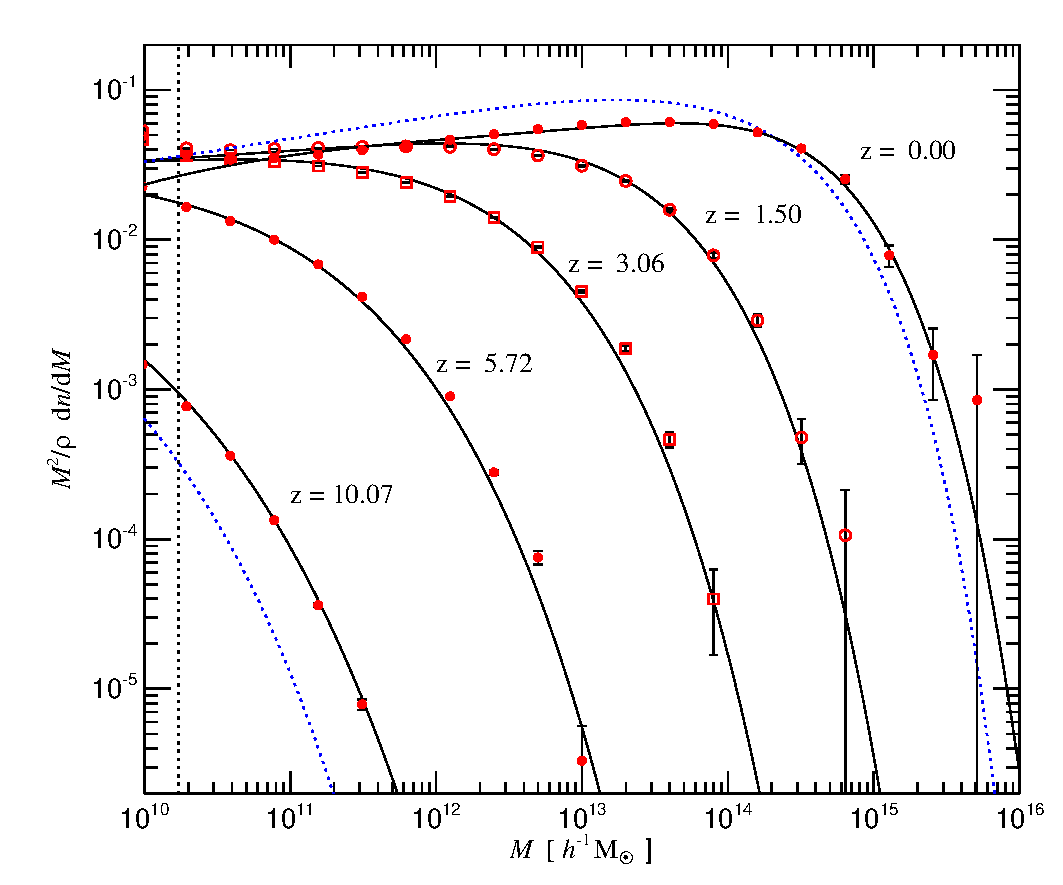
\includegraphics[scale=0.6]{Struct-halo_accretion.pdf}
    \caption{The Millennium Simulation generated number density of halos of 
      baryonic test particles accreting into Dark Matter halos for different 
      eras of redshift, both scales in log. 
    Credit: Springel et al. 2005}
    \label{fig:Struct-halo_accretion}
    \end{centering}
  \end{figure}
  

% 6. Conclusions.
% Providing some concluding remarks and briefly comment on future tests of 
% the standard model.
\section{Conclusion}

  Constraining the free parameters of the physics of the Standard Model to
  fit the best observations of the universe today produces a benchmark model,
  which can be broken down into contributions of different 
  constituents to the energy density of the unverse in the following way,
  (\cite{ryden2003introduction}):

  \begin{center}
  \begin{tabular}{ c c c }
    Photons & \(\Omega_{\gamma} = 5.35E-5 \) \\
    Neutrinos & \(\Omega_{\nu} = 3.65E-5 \) \\
    Total radiation & \(\Omega_{r} = 9.0E-5 \) \\
    Baryonic matter & \(\Omega_{b} = 0.048 \) \\
    Nonbaryonic matter & \(\Omega_{dm} = 0.262 \) \\
    Total matter & \(\Omega_{m} = 0.31 \) \\
    Cosmological constant & \(\Omega_{\Lambda} \approx 0.69 \)
 \end{tabular}
 \end{center}

%TC:ignore

\pagebreak
\begin{singlespace}
\printbibliography
\end{singlespace}

%TC:endignore

\end{document}

